% cd ..\..\Users\NikitaSkybytskyi\Desktop\c3s1\complex-analysis
% cls && pdflatex lec-04.tex && pdflatex lec-04.tex && del lec-04.out, lec-04.log, lec-04.aux && start lec-04.pdf

% \documentclass[a4paper, 12pt]{article}
\usepackage[utf8]{inputenc}
\usepackage[english, ukrainian]{babel}

\usepackage{amsmath, amssymb}
\usepackage{multicol}
\usepackage{graphicx}
\usepackage{float}

\usepackage{amsthm}
\newtheorem{theorem}{Теорема}[subsection]
\newtheorem*{theorem*}{Теорема}
\newtheorem{lemma}{Лема}[subsection]
\newtheorem*{lemma*}{Лема}
\theoremstyle{definition}
\newtheorem*{remark*}{Зауваження}
\newtheorem*{example}{Приклад}

\newcommand{\Max}{\max\limits}
\newcommand{\Sum}{\sum\limits}
\newcommand{\Int}{\int\limits}
\newcommand{\Lim}{\lim\limits}

\newcommand{\RR}{\mathbb{R}}
\newcommand{\ZZ}{\mathbb{Z}}

\newcommand*\diff{\mathop{}\!\mathrm{d}}
\newcommand*\Diff[1]{\mathop{}\!\mathrm{d^#1}}

\DeclareMathOperator{\Real}{Re}
\DeclareMathOperator{\Imag}{Im}

\DeclareMathOperator{\Ln}{Ln}

\DeclareMathOperator{\Arg}{Arg}

\DeclareMathOperator{\Arctan}{Arctan}
\DeclareMathOperator{\Arcsin}{Arcsin}
\DeclareMathOperator{\Arccos}{Arccos}
\DeclareMathOperator{\Arccosh}{Arccosh}
\DeclareMathOperator{\Arctanh}{Arctanh}

\DeclareMathOperator{\arcsinh}{arcsinh}
\DeclareMathOperator{\arccosh}{arccosh}
\DeclareMathOperator{\arctanh}{arctanh}
\DeclareMathOperator{\arccoth}{arccoth}

\newcommand{\varLimsup}{\varlimsup\limits}

\renewcommand{\epsilon}{\varepsilon}
\renewcommand{\phi}{\varphi}

\allowdisplaybreaks
\setlength\parindent{0pt}

\usepackage{xcolor}
\usepackage{hyperref}
\hypersetup{unicode=true,colorlinks=true,linktoc=all,linkcolor=red}

\numberwithin{equation}{section}% reset equation counter for sections
\numberwithin{equation}{subsection}
% Omit `.0` in equation numbers for non-existent subsections.
\renewcommand*{\theequation}{%
  \ifnum\value{subsection}=0 %
    \thesection
  \else
    \thesubsection
  \fi
  .\arabic{equation}%
}


% \begin{document}

\setcounter{section}{3}
\section{Інтегрування функцій комплексної змінної}

У цьому параграфі ми розглянемо поняття інтегралу від функції комплексної змінної та найважливіші властивості аналітичних функції, пов'язані з поняттям інтегралу або такі, що спираються на нього. \\

Зокрема, буде встановлена рівносильність понять про аналітичну функцію як про функцію диференційовну в кожній точці області визначення, і як про функцію, інтеграл від якої не залежить від шляху. \\

Це надає нову концепцію у побудові теорії аналітичних функцій. Застосування поняття інтегралу і теорем, що базуються на ньому, ми розглянемо у наступних главах.

% \setcounter{subsection}{10}
\subsection{Інтеграл від функції комплексної змінної}

Нехай задана деяка орієнтована крива $C$, і визначена на ній функція комплексної змінної $f(z)$. За визначенням, \textit{інтегралом} від $f(z)$ вздовж $C$ називають

\begin{equation}
	\label{eq:4.1.1}
	\Lim_{n \to \infty} \Sum_{k = 0}^{n - 1} f(\zeta_k) \cdot (z_{k + 1} - z_k) = \Int_C f(z) \diff z,
\end{equation}

де $z_0 = a, z_1, \ldots, z_{n + 1} = b$ -- послідовні точки, що розбивають $C$ на $n$ ділянок, через $a$ і $b$ позначені кінці $C$, $\zeta_k$ -- довільна точка що лежить на ділянці $[z_k, z_{k + 1}]$ кривої $C$, і границя береться у припущенні що $\max_k |z_{k + 1} - z_k| \to 0$. \\

Якщо $C$ -- кусково-гладка крива, а $f(z)$ -- кусково-неперервна та обмежена функція, то інтеграл \eqref{eq:4.1.1} завжди існує. Доведення зводиться до відомої з аналізу теореми про існування криволінійного інтеграла від функції дійсної змінної. Справді, поклавши
\begin{equation}
	\label{eq:4.1.2}
	\left\{
		\begin{aligned}
			& f(z) = u(x, y) + i v(x, y), \\
			& z_k = x_k + i y_k, \quad x_{k + 1} - x_k = \Delta x_k, \quad y_{k + 1} - y_k = \Delta y_k, \\
			& \zeta_k = \xi_k + i \eta_k, \quad u(\xi_k, \eta_k) = u_k, \quad v(\xi_k, \eta_k) = v_k,
		\end{aligned}
	\right.
\end{equation}
отримаємо
\begin{equation}
	\label{eq:4.1.3}
	\Sum_{k = 0}^{n - 1} f(\zeta_k) \cdot (z_{k + 1} - z_k) = \Sum_{k = 0}^{n - 1} (u_k \Delta x_k - v_k \Delta y_k) + i \Sum_{k = 0}^{n - 1} (u_k \Delta y_k + v_k \Delta x_k).
\end{equation}

Суми у правій частині \eqref{eq:4.1.3} є інтегральними сумами для відповідних криволінійних інтегралів. У наших умовах ці інтеграли існують і, як наслідок, існує

\begin{equation}
	\label{eq:4.1.4}
	\Int_C f(z) \diff z = \Int_C (u \diff x - v \diff y) + i \Int_C (u \diff y + v \diff x).
\end{equation}

За допомогою формули \eqref{eq:4.1.4} обчислення інтегралу від функції комплексної змінної зводиться до обчислення дійсних інтегралів. \\

Застосовуючи введені визначення, легко бачити, що похідні та інтеграл комплексної функції дійсної змінної $w(t) = \phi(t) + i \psi(t)$ представляються наступними лінійними комбінаціями:
\begin{align}
	\label{eq:4.1.5}
	w'(t) &= \phi'(t) + i \psi'(t), \\
	\label{eq:4.1.6}
	\Int_\alpha^\beta w(t) \diff t &= \Int_\alpha^\beta \phi(t) \diff t + i \Int_\alpha^\beta \psi(t) \diff t.
\end{align}

Нехай $z = z(t) = x(t) + i y(t)$ дає параметричне представлення кривої $C$, причому $z(\alpha) = a$, $z(\beta) = b$. Тоді, користуючись формулою \eqref{eq:4.1.4}, ми зведемо обчислення інтегралу від $f(z)$ вздовж $C$ до обчислення інтегралу від комплексної функції дійсної змінної:
\begin{equation}
	\label{eq:4.1.7}
	\Int_C f(z) \diff z = \Int_\alpha^\beta f(z(t)) \cdot z'(t) \diff t.
\end{equation}

З формули \eqref{eq:4.1.4} також випливає, що на інтеграли від функцій комплексної змінної розповсюджуються звичайні властивості криволінійних інтегралів:
\begin{align}
	\label{eq:4.1.8}
	\Int_C (a \cdot f(z) + b\cdot g(z)) \diff z &= a \Int_C f(z) \diff z + b \Int_C g(z) \diff z, \\
	\label{eq:4.1.9}
	\Int_{C_1 + C_2} f(z) \diff z &= \Int_{C_1} f(z) \diff z + \Int_{C_2} f(z) \diff z, \\
	\label{eq:4.1.10}
	\Int_C f(z) \diff z &= - \Int_{C^-} f(z) \diff z,
\end{align}
де $a$ і $b$ -- комплексні числа, через $C_1 + C_2$ позначена крива що складається з $C_1$ і $C_2$, а через $C^-$ -- крива, що збігається з $C$, але проходиться у зворотному напрямку. \\

Доведемо ще одну властивість інтегралу: нехай $M = \Max_C |f(z)|$, $l$ -- довжина $C$, тоді
\begin{equation}
	\label{eq:4.1.11}
	\left| \Int_C f(z) \diff z \right| \le \Int_C |f(z)| \cdot |\diff z| \le M l.
\end{equation}

Доведення випливає безпосередньо з визначення інтегралу. Справді, маємо:
\begin{equation}
	\label{eq:4.1.12}
	\left| \Sum_{k = 0}^{n - 1} f(\zeta_k) \cdot\Delta z_k \right| \le \Sum_{k = 0}^{n - 1} |f(\zeta_k) |\cdot |\Delta z_k| \le M \Sum_{k = 0}^{n - 1} |\Delta z_k|,
\end{equation}

де $\sum_{k = 0}^{n - 1} |\Delta z_k|$ -- довжина ламаної $z_0 z_1 \ldots z_n$ що вписана у криву $C$. \\

Перейшовши до границі при $|\Delta z_k| \to 0$ отримаємо \eqref{eq:4.1.11}.

% \setcounter{subsection}{11}
\subsection{Теорема Коші}
У загальному випадку $\int_C f(z) \diff z$ залежить як від підінтегральної функції $f(z)$ так і від кривої $C$. Однак, якщо функція $f(z)$ аналітична у деякій однозв'язній області, що містить криву $C$, то інтеграл цілком визначається положенням кінців $C$ і не залежить від вигляду цієї лінії. Іншими словами, справджується

\begin{theorem}[О. Коші, 1825 р.]
\label{th:4.2.1}
Якщо функція $f(z)$ аналітична в однозв'язній області $D$, то для всіх кривих $C$, що лежать у цій області та мають спільні кінці, інтеграл $\int_C f(z) \diff z$ набуває одного і того ж значення.
\end{theorem}

Ми доведемо цю теорему у додатковому припущенні неперервності похідної $f'(z)$.

\begin{proof}
Нехай, як завжди, $f(z) = u(x, y) + i v(x, y)$. Завдяки співвідношенню
\begin{equation}
\label{eq:4.2.1}
\Int_C f(z) \diff z = \Int_C (u \diff x - v \diff y) + i \Int_C (u \diff y + v \diff x).
\end{equation}
(див. також \eqref{eq:4.1.4}, питання про незалежність інтегралу $\int_C f(z) \diff z$ від шляху зводиться до питання про незалежність від шляху криволінійних інтегралів
\begin{equation}
\label{eq:4.2.2}
\Int_C (u \diff x - v \diff y), \quad \Int_C (u \diff y + v \diff x).
\end{equation}
Але, як відомо з аналізу, в однозв'язній області для незалежності від шляху криволінійного інтеграла $\int_C (P \diff x + Q \diff y)$, де $P$ і $Q$ -- функції, що мають неперервні частинні похідні, необхідно і достатньо, аби підінтегральний вираз був повним диференціалом, тобто аби у кожній точці області $D$ виконувалося $\frac{\partial P}{\partial y} = \frac{\partial Q}{\partial x}$. \\

Для інтегралів \eqref{eq:4.2.2} ці співвідношення набувають вигляду
\begin{equation}
\label{eq:4.2.3}
\dfrac{\partial u}{\partial y} = - \dfrac{\partial v}{\partial x}, \quad \dfrac{\partial v}{\partial y} = \dfrac{\partial u}{\partial x},
\end{equation} а неперервність частинних похідних випливає з припущення про неперервність $f'(z)$. Рівняння \eqref{eq:4.2.3} збігаються з умовами Коші-Рімана і задовольняються, оскільки $f(z)$ функція аналітична.
\end{proof}

Завдяки цій теоремі для аналітичних в однозв'язних областях функції, замість $\int_C f(z) \diff z$ можемо писати $\int_{z_0}^z f(\zeta) \diff \zeta$, де через $z_0$ і $z$ позначені кінці кривої $C$. \\

Використовуючи теорему \ref{th:4.2.1} можна довести ряд тверджень аналогічних до звичайних тверджень інтегрального числення. Перш за все, виконується
\begin{theorem}
\label{th:4.2.2}
Якщо функція аналітична в однозв'язній області, то інтеграл
\begin{equation}
\label{eq:4.2.4}
\Int_{z_0}^z f(\zeta) \diff \zeta = F(z),
\end{equation}
що розглядається в залежності від своєї верхньої межі, також є аналітичною функцією, причому
\begin{equation}
\label{eq:4.2.5}
F'(z) = \dfrac{\diff}{\diff z} \Int_{z_0}^z f(\zeta) \diff \zeta = f(z).
\end{equation}
\end{theorem}

\begin{proof}
Справді, за визначенням похідної і властивостями інтегралу \eqref{eq:4.1.9} і \eqref{eq:4.1.10} маємо
\begin{multline}
\label{eq:4.2.6}
F'(z) = \Lim_{h \to 0} \dfrac{F(z + h) - F(z)}{h} = \Lim_{h \to 0} \dfrac{1}{h} \left( \Int_{z_0}^{z + h} f(\zeta) \diff \zeta - \Int_{z_0}^z f(\zeta) \diff \zeta \right) = \\
= \Lim_{h \to 0} \dfrac{1}{h} \Int_z^{z + h} d(\zeta) \diff \zeta.
\end{multline}

Завдяки неперервності $f(z)$ в точці $z$ можемо записати:
\begin{equation*}
f(\zeta) = f(z) + \eta (\zeta),
\end{equation*}
де $\eta(\zeta) \to 0$ при $\zeta \to z$. Підставляючи це у \eqref{eq:4.2.6}, отримаємо
\begin{equation}
\label{eq:4.2.7}
F'(z) = \Lim_{h \to 0} \dfrac{1}{h} \Int_z^{z + h} f(z) \diff \zeta + \Lim_{h \to 0} \dfrac{1}{h} \Int_z^{z + h} \eta(z) \diff \zeta.
\end{equation}

Оскільки $f(z)$ -- величина стала при інтегруванні за $\zeta$, то
\begin{equation}
	\label{eq:4.2.8}
	\Int_z^{z + h} f(z) \diff \zeta = f(z) \Int_z^{z + h} \diff \zeta = h \cdot f(z),
\end{equation}
адже з визначення безпосередньо випливає, що $\int_z^{z + h} \diff \zeta = h$. \\

Далі, з нерівності \eqref{eq:4.1.11} маємо
\begin{equation}
	\label{eq:4.2.9}
	\left| \Int_z^{z + h} \eta(\zeta) \diff \zeta \right| \le |h| \cdot \Max |\eta(\zeta)|
\end{equation}
(шлях інтегрування від точки $z$ до точки $z + h$ за теоремою \ref{th:4.2.1} можна вважати прямолінійним, тому його довжина дорівнює $|h|$). Таким чином, в \eqref{eq:4.2.7} перша границя дорівнює $f(z)$, а друга -- нулю, тобто $F'(z) = f(z)$, що і потрібно було довести.
\end{proof}

Функція, чия похідна дорівнює заданій функції $f(z)$ називається \textit{первісною} цієї функції. Щойно доведена теорема стверджує, що інтеграл від $f(z)$ який розглядається фу функція своєї верхньої межі, є однією з первісних функції $f(z)$.

\begin{theorem}
	\label{th:4.2.3}
	Довільні дві первісні однієї й тієї ж функції відрізняються одна від одної не більш ніж на сталий доданок.
\end{theorem}

\begin{proof}
Нехай $F_1(z)$ і $F_2(z)$ -- ці первісні, і
\begin{equation}
	\label{eq:4.2.10}
	\Phi(z) = F_1(z) - F_2(z) = u(x, y) + i v(x, y).
\end{equation}
Для доведення теореми достатньо показати, що функція $\Phi(z)$ стала. \\

За формулою для похідної, маємо:
\begin{equation}
	\label{eq:4.2.11}
	\Phi'(z) = \dfrac{\partial u}{\partial x} + i \dfrac{\partial v}{\partial x} = \dfrac{\partial v}{\partial y} - i \dfrac{\partial u}{\partial y} \equiv 0,
\end{equation}
адже за нашою умовою $\Phi'(z) = F_1'(z) - F_2'(z) = f(z) - f(z) = 0$. \\

Звідси випливає, що $\frac{\partial u}{\partial x} = \frac{\partial v}{\partial y} \equiv 0$, $\frac{\partial v}{\partial x} = \frac{\partial u}{\partial y} \equiv 0$, тому $u(x, y)$ і $v(x, y)$ сталі.
\end{proof}

Наступна теорема дозволяє обчислювати інтеграл за допомогою первісних.

\begin{theorem}
	\label{th:4.2.4}
	Якщо $F(z)$ -- довільна первісна аналітичної функції $f(z)$, то
	\begin{equation}
		\label{eq:4.2.12}
		\Int_{z_0}^z f(\zeta) \diff \zeta = F(z) - F(z_0).
	\end{equation}
\end{theorem}

\begin{proof}
Справді, за теоремою \ref{th:4.2.2}, функція $F_1(z) = \int_{z_0}^z f(\zeta) \diff \zeta$ є однією з первісних для $f(z)$, а функція $F(z)$ також первісна, тому, за теоремою \ref{th:4.2.3},
\begin{equation}
	\label{eq:4.2.13}
	\Int_{z_0}^z f(\zeta) \diff \zeta = F(z) + C,
\end{equation}
де $C$ -- деяка стала. Покладаючи у цій рівності $z = z_0$, знаходимо $F(z_0) + C = 0$, звідки $C = - F(z_0)$, що і дає шукану формулу \eqref{eq:4.2.12}.
\end{proof}

Зауважимо також, що теоремі Коші, доведеній на початку цього пункту можна надати наступного вигляду:
\begin{theorem*}
Якщо функція $f(z)$ аналітична в однозв'язній області $D$, то її інтеграл вздовж довільного замкнутого контура $C$, що лежить в $D$ дорівнює нулеві:
	\begin{equation}
	\label{eq:4.2.14}
	\Int_C f(z) \diff z = 0.
	\end{equation}
\end{theorem*}

Доведення спирається на те, що замкнутий контур $C$ можна розкласти на два шляхи, $C_1$ і $C_2$ зі спільними початком і кінцем:
\begin{figure}[H]
	\centering
	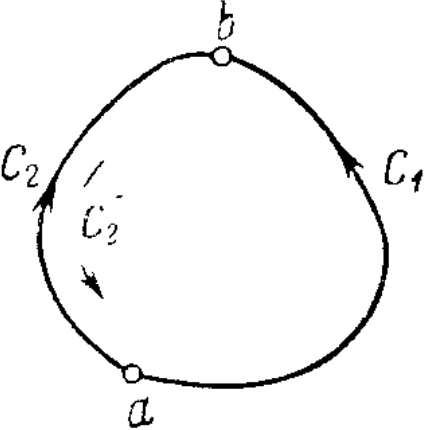
\includegraphics[width=.4\linewidth]{mal-18.png}
	%\caption{Розбиття контуру на два шляхи зі спільними початком і кінцем.}
\end{figure}

За властивостями інтегралів,
\begin{equation}
	\label{eq:4.2.15}
	\Int_C f(z) \diff z = \Int_{C_1} f(z) \diff z + \Int_{C_2^-} f(z) \diff z = \Int_{C_1} f(z) \diff z - \Int_{C_2} f(z) \diff z.
\end{equation}
Як наслідок, рівність нулю інтегралу вздовж $C$ рівносильне рівності між собою інтегралів вздовж $C_1$ та $C_2$. \\

На завершення доведемо ще одне корисну для подальшого застосування узагальнення теореми Коші. А саме, в теоремі Коші (в останньому формулюванні) мова йде про інтегра по контуру, який цілком лежить всередині області аналітичності функції, хоча інколи доводиться розглядати інтеграли вздовж кривих, на яких функція, залишаючись неперервною, перестає бути аналітичною. Виявляється, теорема Коші залишається в силі і для цього випадку:

\begin{theorem}
	\label{th:4.2.5}
	Якщо функція $f(z)$ аналітична в однозв'язній області $D$ і неперервна в замкнутій області $\overline{D}$, то інтеграл від $f(z)$ взятий вздовж границі $C$ цієї області дорівнює нулю:
	\begin{equation}
		\label{eq:4.2.16}
		\Int_C f(z) \diff z = 0.
	\end{equation}
\end{theorem}
\begin{proof}
	Припустимо для початку, що $C$ є ``зоряний'' контур, тобто існує точка $z_0$ така, що довільний промінь з вершиною в цій точці перетинає $C$ в одній і тільки в одній точці. Без обмеження загальності можна вважати, що $z_0 = 0$, тоді криву $C$ можна задати рівнянням $z = r(\phi) \cdot e^{i \phi}$, де $r(\phi)$ -- однозначна функція. \\

	Позначимо контур, що визначається рівнянням $\zeta = \lambda z = \lambda \cdot r(\phi) \cdot e^{i \phi}$, $0 < \lambda < 1$, як $C_\lambda$:
	\begin{figure}[H]
		\centering
		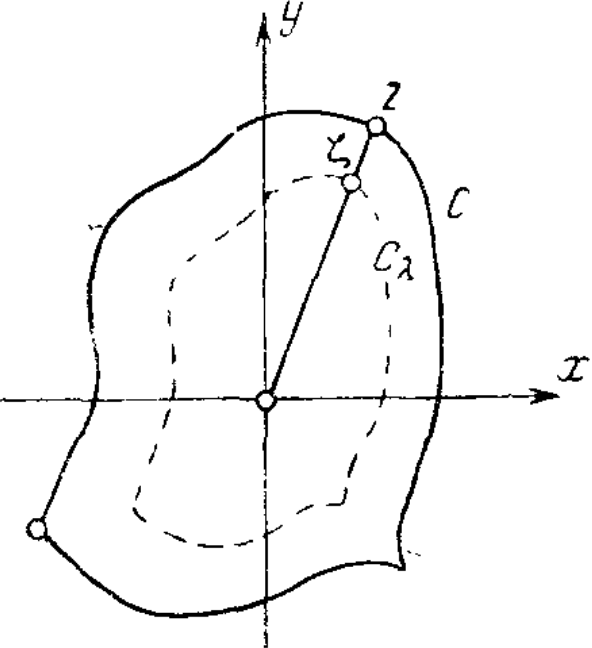
\includegraphics[width=.4\linewidth]{mal-19.png}
	\end{figure}

	Оскільки $C_\lambda$ лежить всередині $D$, то, за теоремою Коші,
	\begin{equation}
		\label{eq:4.2.17}
		\Int_{C_\lambda} f(\zeta) \cdot \diff \zeta = 0.
	\end{equation}

	Але коли точка $\zeta$ описує $C_\lambda$, точка $z = \zeta / \lambda$ описує $C$, тому рівність \eqref{eq:4.2.17} можна переписати у вигляді
	\begin{equation}
		\label{eq:4.2.18}
		\Int_C f(\lambda z) \cdot \diff (\lambda z) = \lambda \Int_C f(\lambda z) \cdot \diff z = 0,
	\end{equation}
	і, як наслідок,
	\begin{equation}
		\label{eq:4.2.19}
		\Int_C f(z) \cdot \diff z = \Int_C (f(z) - f(\lambda z)) \cdot \diff z.
	\end{equation}
	Оскільки функція $f(z)$ рівномірно непервна на $\bar D$, то для довільного $\epsilon > 0$ можна знайти $\delta > 0$ таке, що для довільної пари точок $z, \zeta$, які задовольняють нерівності $|z-\zeta|<\delta$ буде виконуватися нерівність 
	\begin{equation}
		\label{eq:4.2.20}
		|f(z) - f(\zeta)| < \epsilon.
	\end{equation}

	Нехай $\ell$ -- довжина контура $C$ і $R = \max r(\phi)$. Візьмемо $\lambda > 1 - \delta / R$, тоді для довільної пари точок $z$ і $\zeta = \lambda z$ будемо мати $|z - \zeta| = (1 - \lambda) \cdot |z| \le \delta / R \cdot |z| \le \delta$, і, як наслідок, буде виконуватися \eqref{eq:4.2.20}. \\

	Тоді з \eqref{eq:4.2.19} отримаємо
	\begin{equation}
		\label{eq:4.2.21}
		\left|\Int_C f(z)\diff z\right| < \ell \epsilon.
	\end{equation}

	Оскільки тут $\epsilon$ як завгодно мале і інтеграл не залежить від $\epsilon$, то цей інтеграл дорівнює нулю. Для ``зоряних'' контурів теорема доведена. \\

	Нехай тепер $C$ -- довільна кусково-гладка крива. Якщо $C$ має точки повернення, то ми викинемо з області $D$ круги малого радіусу $\epsilon$ з центро у цих точках так, щоб границя отриманої області $D_\epsilon$ вже не мала таких точок:
	\begin{figure}[H]
		\centering
		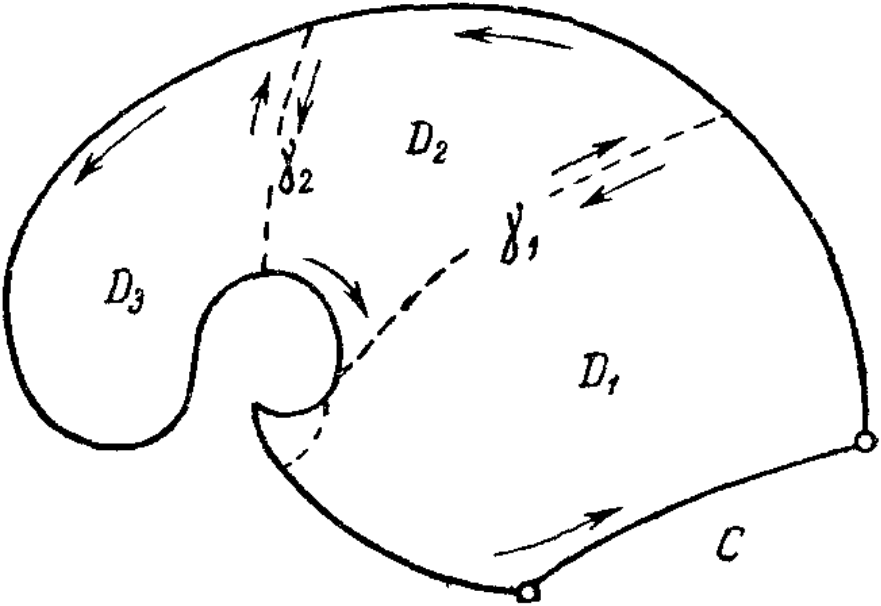
\includegraphics[width=.4\linewidth]{mal-20.png}
	\end{figure}

	Проводячи всередині $D_\epsilon$ скінченну кількість ліній $\gamma_k$ ($k=1,2,\ldots,m$) цю область можна розбити на частини $D_k$ ($k=1,2,\ldots,n$), що обмежені ``зоряними'' контурами $C_k$ ($k=1,2,\ldots,n$). Тоді, за щойно доведеним
	\begin{equation}
		\label{eq:4.2.22}
		\Int_{C_k} f(z) \diff z = 0, \quad (k = 1, 2, \ldots, n).
	\end{equation}

	Припускаючи, що всі лінії $C_k$ проходяться в одному і тому ж напрямку (наприклад у додатному), додамо всі рівності \eqref{eq:4.2.22}, тоді інтеграли вздовж $\gamma_k$ скоротяться (бо кожна така лінія проходиться двічі, у різних напрямках), і отримаємо 
	\begin{equation}
		\label{eq:4.2.23}
		\Int_{C_\epsilon} f(z) \diff z = 0.
	\end{equation}

	Залишається довести, що інтеграл вздовж границі початкової області також дорівнює нулю, але це безпосередньо випливає з того, що $C$ і $C_\epsilon$ відрізняються лише на скінченну кількість нескінченно малих дуг, а функція $f$ обмежена, тому $\int_{C_\epsilon} \to \int_C$ при $\epsilon\to0$.
\end{proof}

% \setcounter{subsection}{12}
\subsection{Розповсюдження на багатозв'язні області}
Для багатозв'язних областей теорема Коші, взагалі кажучи, не виконується. Справді, функція $f(z) = 1 / z$ аналітична всюди у кільці $\frac{1}{2} < |z| < 2$, одначе інтеграли від $-1$ до $1$ вздовж верхньої та нижньої половин кола $|z| = 1$ відрізняються. \\

Справді, вздовж верхнього півкола $C_1$, де $z = e^{i \phi}$, $0 < \phi < \pi$, ми маємо:
\begin{equation}
	\label{eq:4.3.1}
	\Int_{C_1} \dfrac{\diff z}{z} = \Int_\pi^0 \dfrac{i e^{i \phi} \diff \phi}{e^{i \phi}} = - i \pi,
\end{equation} а вздовж нижнього півкола $C_2$, де $z = e^{i \phi}$, $-\pi < \phi < 0$, ми маємо:
\begin{equation}
	\label{eq:4.3.2}
	\Int_{C_2} \dfrac{\diff z}{z} = \Int_{-\pi}^0 \dfrac{i e^{i \phi} \diff \phi}{e^{i \phi}} = i \pi.
\end{equation}

Через це ми будемо інколи використовувати символ
\begin{equation}
	\label{eq:4.3.3}
	\Int_{a^C}^b f(z) \diff z.
\end{equation}
для позначення інтегралу від $a$ до $b$ вздовж шляху $C$ у багатозв'язній області. \\

Нехай в багатозв'язній області $D$ задані точки $a$ і $b$ і проста крива $C_0$ що їх з'єднує. Нехай $C$ -- довільна інша крива, що з'єднує ці точки (див. мал. нижче). Згідно тільки-но зробленого зауваження, можна, не змінюючи величини інтегралу, деформувати криву $C$ в іншу криву $\widetilde{C}$, що лежить в області $D$, яка складається з:
\begin{enumerate}
\item кривої $\widetilde{C}_0$, яка разом з $C_0$ обмежує однозв'язну область що належить $D$;
\item сукупності простих замкнутих кривих $\gamma_k$ ($k = 1, 2, \ldots, m$), кожна з яких містить всередині себе одну зв'язну частину границі $D$:
\end{enumerate}

\begin{figure}[H]
	\centering
	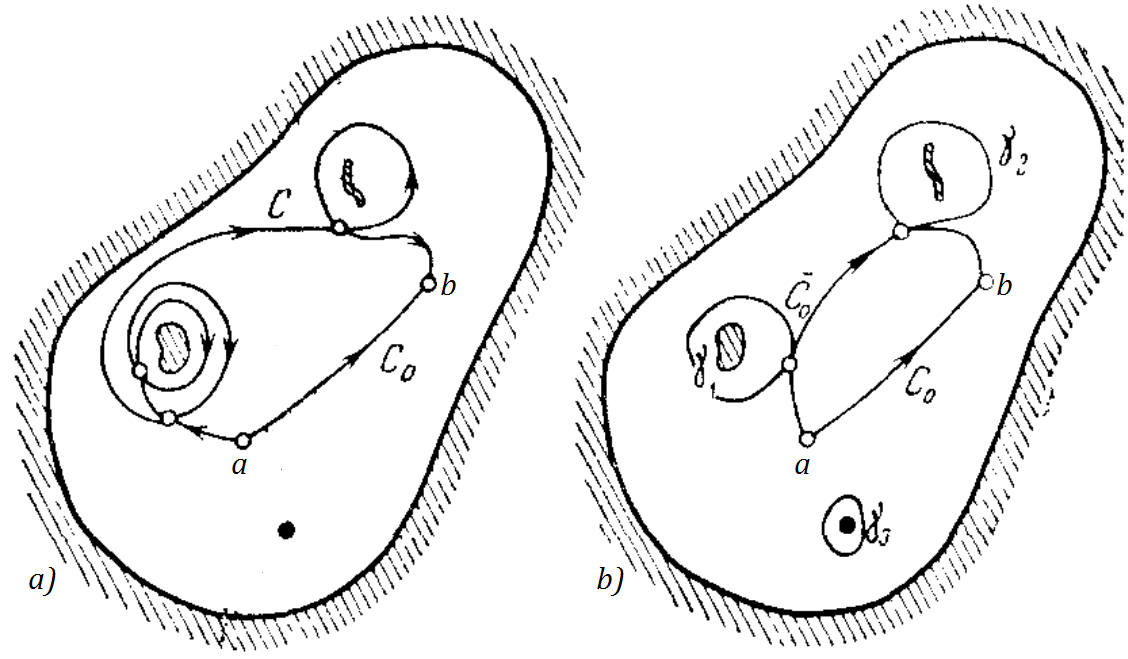
\includegraphics[width=.8\linewidth]{mal-21.png}
	%\caption{Деформація кривої $C$ у криву $\widetilde{C}$.}
\end{figure}

При цьому криві $\gamma_k$ можуть проходитися декілька разів і у різних напрямках. \\

Для зручності, домовимося позначати через $\gamma_k$ ($k = 1, 2, \ldots, m$) криві, що проходяться проти годинникової стрілки. Окрім цього, введемо ще криві $\gamma_k$ ($k = m + 1, \ldots, n$), що обмежують зв'язні частини границі області $D$ і не входять у склад $\widetilde{C}$ (як $\gamma_3$ на мал. вище). \\

Введемо позначення
\begin{equation}
	\label{eq:4.3.4}
	\Gamma_k = \Int_{\gamma_k} f(z) \diff z \quad (k = 1, 2, \ldots, n).
\end{equation}
За неперервної деформації $\gamma_k$ за якої ці криві залишаються всередині $D$, інтеграли \eqref{eq:4.3.4} не змінюються. Як наслідок, величини $\Gamma_k$ визначають лише функцією $f(z)$ і областю $D$. \\

Нехай $N_k$ -- цілі числа, які вказують, скільки разів і в якому напрямку проходиться $\gamma_k$ у складі кривої $\widetilde{C}$. За попереднім спостереженням і властивостями інтегралів \eqref{eq:4.1.9} і \eqref{eq:4.1.10}, маємо:
\begin{equation}
	\label{eq:4.3.5}
	\Int_{a^C}^b f(z) \diff z = \Int_{a^{\widetilde{C}}}^b f(z) \diff z = \Int_{a^{C_0}}^b f(z) \diff z + N_1 \Gamma_1 + N_2 \Gamma_2 + \ldots + N_n \Gamma_n.
\end{equation}
Величини $\Gamma_k$ називаються \textit{періодами інтегралу} від функції $f(z)$ у багатозв'язній області $D$ або \textit{циклічними сталими}. \\
\begin{example}
	Нехай $f(z) = 1 /z$ і $D$ -- ``кільце'' $0 < |z| < R$, де $R$ -- як завгодно велике число. Довільний шлях $C$, що з'єднує точки 1 і $z$, можна, як описано вище, двеформувати у шлях $\tilde C$, який складається з одиничного кола $|z|=1$ (яке, взагалі кажучи, проходиться кілька разів) і простої лінії $C_0$, яка з'єднує точки 1 і $z$:
	\begin{figure}[H]
		\centering
		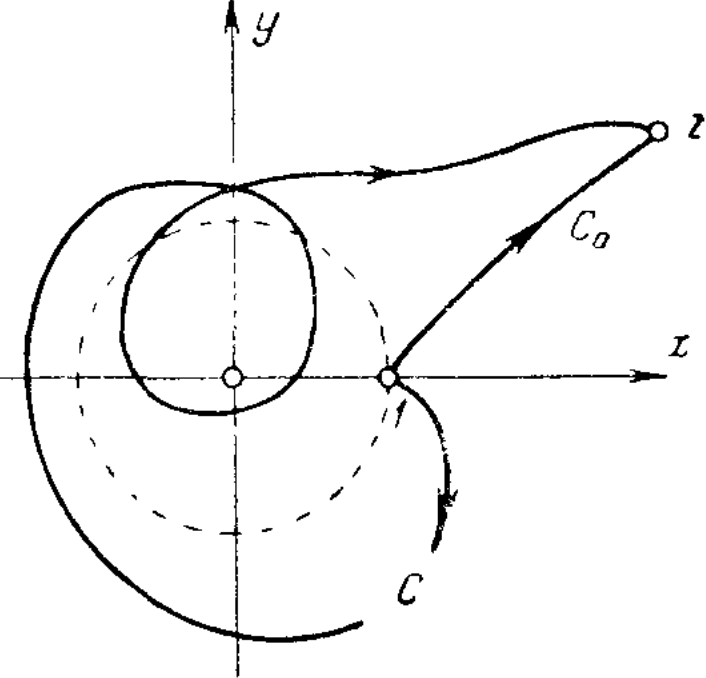
\includegraphics[width=.4\linewidth]{mal-22.png}
	\end{figure}

	Інтеграл вздовж кола, яке проходиться проти годинникової стрілки, тобто коли $z = e^{i \phi}$ і $\phi$ збільшується від $0$ да $2\pi$ дорівнює
	\begin{equation}
		\label{eq:4.3.6}
		\Gamma = \Int_{|z|=1} \frac{\diff}{z} = \Int_0^{2\pi} \frac{e^{i\phi}i\diff\phi}{e^{i\phi}}=2\pi i.
	\end{equation}

	Тоді за формулою \eqref{eq:4.3.5},
	\begin{equation}
		\label{eq:4.3.7}
		\Int_{1^C}^z \frac{\diff z}{z} = \Int_{1^{C_0}}^z \frac{\diff z}{z} + 2 k \pi i,
	\end{equation}
	де $k$ -- ціле число, яке показує, скільки разів (і в якому напрямку) проходиться коло $|z|=1$ у складі $\tilde C$ (на малюнку вище $k=-2$). \\

	За теоремою \ref{th:4.2.4}, 
	\begin{equation}
		\label{eq:4.3.8}
		\Int_{1^{C_0}}^z \frac{\diff z}{z} = \ln \zeta|_{\zeta=1}^{\zeta=z} = \ln z,
	\end{equation}
	де $\ln$ позначає те значення логарифму, яке дорівнює 0 в точці $\zeta = 1$ і непрервно змінюється вздовж $C_0$. \\

	Враховуючи, що $C$ -- довільний шлях, і позначаючи значення інтегралу від $1/z$ вздовж нього через $\Ln z$, ми отримаємо з \eqref{eq:4.3.8}:
	\begin{equation}
		\label{eq:4.3.9}
		\Ln z = \Int_{1^C}^z \frac{\diff z}{z} = \ln z + 2 k \pi i.
	\end{equation}

	Таким чином, ми знову прийшли до багатозначної функції $\Ln z$ і з'ясували природу її багатозначності з нової точки зору.
\end{example}

Зазначимо також, що теоремі Коші минулого пункту можна надати трохи інший сенс так, щоб вона залишилася справедливою і для багатозв'язних областей. Нехай функція $f(z)$ аналітична в багатозв'язній області $D$, обмеженій кривими $C_0, C_1, \ldots, C_n$ і неперервна в $\overline{D}$. Проведемо розрізи $\gamma_1, \ldots, \gamma_n$, що перетворюють $D$ в однозв'язну область $D^*$, і позначимо через $C^*$ границю цієї області -- криву, що складається з частин кривих $C_k$ і кривих $\gamma_k$, причому останні проходяться двічі у протилежних напрямках:

\begin{figure}[H]
	\centering
	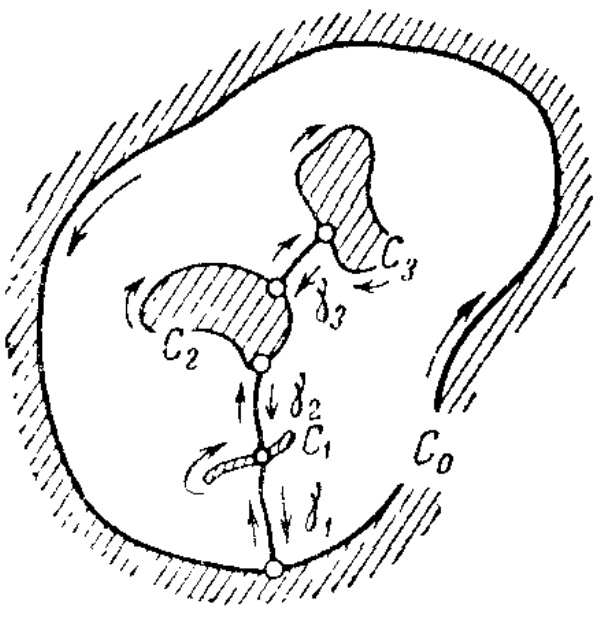
\includegraphics[width=.4\linewidth]{mal-23.png}
	%\caption{Перетворення багатозв'язної області в однозв'язну.}
\end{figure}

Функція $f(z)$ аналітична в однозв'язній області $D^*$ і неперервна в $\overline{D^*}$. Як наслідок, за теоремою \ref{th:4.2.5}, і властивостями інтегралів \eqref{eq:4.1.9} і \eqref{eq:4.1.10}:
\begin{equation}
\label{eq:4.3.10}
\Int_{C^*} f(z) \diff z = \Int_{C_0} f(z) \diff z + \Sum_{k = 1}^n \Int_{C_k} f(z) \diff z = 0,
\end{equation}
де інтеграли вздовж $\gamma_k$ скорочуються, а інша частина $C^*$ збігається з $\sum_{k=0}^n C_k$. \\

При цьому ми маємо вважати, що криві $C_0$ і $C_1, C_2, \ldots, C_n$ обходяться так, аби область $D$ увесь час залишалася з одного боку. Таким чином, для областей довільної зв'язності, теорема Коші виконується у наступному вигляді:
\begin{theorem}
Якщо функція $f(z)$ аналітична в області $D$ і неперервна в $\overline{D}$, то її інтеграл вздовж границі цієї області, яка проходиться так, щоб область $D$ увесь час залишалася з одного боку, дорівнює нулю.
\end{theorem}

% \setcounter{subsection}{13}
\subsection{Формула Коші та теорема про середнє}
Нехай функція $f(z)$ аналітична у $n$-зв'язній області $D$ і неперервна в $\overline{D}$. Покажемо, що для довільної внутрішньої точки $z$ цієї області справджується так звана \textit{формула Коші} (1831 р.):
\begin{equation}
	\label{eq:4.4.1}
	f(z) = \dfrac{1}{2 \pi i} \Int_C \dfrac{f(\zeta) \diff \zeta}{\zeta - z},
\end{equation}
де $C$ -- межа області $D$ що проходиться так, аби область $D$ увесь час залишалася ліворуч. \\

Відзначимо, що у праву частину формули Коші входять лише значення $f(z)$ на границі $C$ області $D$. Таким чином, за зазначених умов значення функції всередині області цілком визначається її значенням на границі: формула Коші дозволяє обчислити значення функції в довільній точці області, якщо відомі межеві значення цієї функції. \\

Для виведення формули Коші ми викинемо з області $D$ круг радіусу $r$ з центром в точці $z$ і помітимо, що в отриманій $(n+1)$-зв'язній області $D^*$ чисельних і знаменник підінтегральної функції аналітичні відносно змінної $\zeta$, причому знаменник не обертається на нуль. Як наслідок, підінтегральна функція аналітична відносно $\zeta$ в $D^*$. Оскільки вона неперервна в $\overline{D^*}$, то за теоремою Коші попереднього пункту:
\begin{equation}
	\label{eq:4.4.2}
	\Int_C \dfrac{f(\zeta) \diff \zeta}{\zeta - z} + \Int_{\gamma_r^-} \dfrac{f(\zeta) \diff \zeta}{\zeta - z} = 0,
\end{equation}
де коло $\gamma_r^-$ проходиться за годинниковою стрілкою. Звідси випливає, що
\begin{equation}
	\label{eq:4.4.3}
	\Int_C \dfrac{f(\zeta) \diff \zeta}{\zeta - z} = \Int_{\gamma_r} \dfrac{f(\zeta) \diff \zeta}{\zeta - z},
\end{equation}
де $\gamma_r$ проходиться проти годинникової стрілки. На колі $\gamma_r$ маємо $\zeta - z = re^{i \phi}$, тому, виносячи за знак інтегралу сталий відносно $\zeta$ множини $f(z)$, знаходимо
\begin{equation}
	\label{eq:4.4.4}
	\dfrac{1}{2 \pi i} \Int_{\gamma_r} \dfrac{f(z) \diff \zeta}{\zeta - z} = \dfrac{f(z)}{2 \pi i} \Int_0^{2 \pi} \dfrac{r i e^{i \phi} \diff \phi}{r e^{i \phi}} = f(z).
\end{equation}
З формул \eqref{eq:4.4.3} і \eqref{eq:4.4.4} маємо:
\begin{equation}
	\label{eq:4.4.5}
	\dfrac{1}{2 \pi i} \Int_C \dfrac{f(\zeta) \diff \zeta}{\zeta - z} - f(z) = \dfrac{1}{2 \pi i} \Int_{\gamma_r} \dfrac{f(\zeta) - f(z)}{\zeta - z} \diff \zeta.
\end{equation}
Оцінимо цю різницю. Згідно з нерівністю \eqref{eq:4.1.11}:
\begin{multline}
	\label{eq:4.4.6}
	\left| \dfrac{1}{2 \pi i} \Int_{\gamma_r} \dfrac{f(\zeta) - f(z)}{\zeta - z} \diff \zeta \right| \le \dfrac{1}{2 \pi} \Max_{\gamma_r} |f(\zeta) - f(z)| \dfrac{2 \pi r}{r} = \\ = \Max_{\gamma_r} |f(\zeta) - f(z)| \xrightarrow[r \to 0]{} 0.
\end{multline}
З іншого боку, як видно з лівої частини \eqref{eq:4.4.5}, ця різниця не залежить від $r$, отже вона має дорівнювати нулю, і формула Коші доведена. \\

Якщо, зокрема, крива $C$ являє собою коло $|\zeta - z| = R$, то, покладаючи $\zeta - z = R e^{i \phi}$ ми отримаємо з формули Коші
\begin{equation}
	\label{eq:4.4.7}
	f(z) = \dfrac{1}{2 \pi} \Int_0^{2 \pi} f(z + R e^{i \phi}) \diff \phi.
\end{equation}

Остання формула виражає \textit{теорему про середнє} для аналітичних функцій:
\begin{theorem}
Якщо функція $f(z)$ неперервна в замкнутому крузі і аналітична всередині цього круга, то її значення у центрі круга дорівнює середньому арифметичному її значень на колі.
\end{theorem}

% \setcounter{subsection}{14}
\subsection{Принцип максимуму і лема Шварца}
Спершу доведемо одну просту лему.
\begin{lemma}
	Якщо в деякій області $D$:
	\begin{enumerate}
		\item стала дійсна частина аналітичної функції $f(z)$ або
		\item сталий її модуль
	\end{enumerate}
	то і сама ця функція стала.
\end{lemma}

\begin{proof}
За першої умови твердження випливає безпосередньо з рівнянь Коші-Рімана: у нас 
\begin{equation}
	\label{eq:4.5.1}
	\frac{\partial u}{\partial x} = \frac{\partial u}{\partial y} \equiv 0,
\end{equation} як наслідок, в силу цих рівнянь і
\begin{equation}
 	\label{eq:4.5.2}
 	\frac{\partial v}{\partial x} = \frac{\partial v}{\partial y} \equiv 0.
\end{equation}

Звідси робимо висновок, що $v$, а отже і функція $f(z)$, стала в області $D$. \\

Перейдемо до доведення леми за другої умови. Нехай $|f(z)| \equiv M$, де $M$ -- стала. Для $M = 0$ твердження леми очевидне. Якщо ж $M \ne 0$, то ми розглянемо функцію
\begin{equation}
	\label{eq:4.5.3}
	\ln f(z) = \ln |f(z)| + i \arg f(z),
\end{equation}
яка у цьому випадку аналітична. Її дійсна частина стала ($= \ln M$). Як наслідок, за вже доведеною частиною леми, стала сама функція $\ln f(z)$, а отже і $f(z)$.
\end{proof}

Доведемо тепер \textit{принцип максимуму модуля} для аналітичних функцій.

\begin{theorem}
	Якщо функція $f(z)$, не дорівнює тотожно сталій, аналітична в області $D$ і неперервна в $\overline{D}$, то її модуль не може досягати найбільшого значення у внутрішній точці області $D$.
\end{theorem}

\begin{proof}
В силу властивостей неперервних функцій, $|f(z)|$ досягає свого максимуму $M$ всередині або на границі $D$. Припустимо від супротивного, що $|f(z)|$ досягає значення $M$ всередині $D$, і позначимо через $\mathcal{E}$ множину всіх точок $D$ для яких $|f(z)| = M$. Якщо $\mathcal{E} = \overline{D}$, то всюди в $D$ маємо $|f(z)| = M$, тобто $|f(z)|$ сталий. Звідси за лемою випливає, що і $f(z)$ стала в $D$, а це суперечить умовам теореми. \\

Якщо ж $\mathcal{E}$ не збігається з $D$, то існує гранична точка $z_0$ цієї множини яка є внутрішньою точкою $D$. В силу неперервності $f(z)$ маємо $|f(z_0)| = M$, адже в довільному околі $z_0$ є точки $\mathcal{E}$. Побудуємо коло $C: |z - z_0| = r$, що належить області $D$, так, щоб на ній була хоча б одна точка $z_1$ що не належить множині $\mathcal{E}$. (Це завжди можна зробити, адже $z_0$ -- гранична точка $\mathcal{E}$). Тоді $|f(z_1)| < M$ і для довільного достатньо малого $\epsilon > 0$, в силу неперервності $f(z)$, завжди можна знайти таку частину $C_1$ кола $C$ яка містить точку $z_1$ на якій
\begin{equation}
	\label{eq:4.5.4}
	|f(z)| < M - \epsilon.
\end{equation}
Позначимо через $C_2$ решту кола. На ній, очевидно,
\begin{equation}
	\label{eq:4.5.5}
	|f(z)| \le M.
\end{equation}
За теоремою про середнє, маємо:
\begin{equation}
\label{eq:4.5.6}
	f(z_0) = \dfrac{1}{2 \pi} \Int_0^{2 \pi} f(z) \diff \phi = \dfrac{1}{2 \pi r} \left(\Int_{C_1} f(z) \diff s + \Int_{C_2} f(z) \diff s \right),
\end{equation}
де $\diff s = r \diff \phi$ -- елемент довжини кола $C$. \\

Переходячи у співвідношенні \eqref{eq:4.5.6} до абсолютних величин і враховуючи нерівності \eqref{eq:4.5.4} і \eqref{eq:4.5.5}, отримаємо
\begin{equation}
	\label{eq:4.5.7}
	M = |f(z_0)| \le \dfrac{1}{2 \pi r} ((M - \epsilon) l_1 + M l_2) = M - \dfrac{\epsilon l_1}{2 \pi r},
\end{equation}
де $l_1$ і $l_2$ -- довжини $C_1$ і $C_2$ відповідно ($l_1 + l_2 = 2 \pi r$). Але остання нерівність неможлива, чим і доводиться наш принцип.
\end{proof}

\begin{remark*}
	Якщо функція $f(z)$ не стала, аналітична в $D$ і неперервна в $\overline{D}$ і, окрім цього, не обертається на 0, то і мінімум $|f(z)|$ не може досягатися всередині $D$.
\end{remark*}
Для доведення достатньо застосувати принцип максимуму до функції $g(z) = 1 / f(z)$. \\

З принципу максимуму модуля випливає корисна для подальших застосувань
\begin{lemma}[Г. Шварц]
	Якщо функція $f(z)$ аналітична в крузі $|z| < 1$ і неперервна в замкнутому крузі, причому $f(0) = 0$, і якщо всюди в крузі $|f(z)| \le 1$, то у цьому ж крузі
	\begin{equation}
		\label{eq:4.5.8}
		|f(z)| \le |z|.
	\end{equation}
	При цьому, якщо хоча б в одній внутрішній точці круга $|f(z) = |z|$, то остання рівність виконується у всьому крузі, і
	\begin{equation}
		\label{eq:4.5.9}
		f(z) = e^{i \alpha} z,
	\end{equation}
	де $\alpha$ -- дійсна стала.
\end{lemma}

\begin{proof}
Для доведення розглянемо функцію
\begin{equation}
	\label{eq:4.5.10}
	\phi(z) = \begin{cases} \dfrac{f(z)}{z} & z \ne 0, \\ f'(0) & z = 0. \end{cases}
\end{equation}
З умов леми випливає, що $\phi(z)$ аналітична у кільці $0 < |z| < 1$ і неперервна в замкнутому крузі $|z| \le 1$. \\

В пункті 22 буде доведено, що звідси випливає аналітичність $\phi(z)$ в точці $z = 0$. Таким чином, до $\phi(z)$ можна застосовувати принцип максимуму модуля. Оскільки на колі $|z| = 1$ маємо $|\phi(z)| = \left| \frac{f(z)}{z} \right| \le 1$, то за цим принципом і всюди в крузі $\phi(z) \le 1$, тобто $|f(z)| \le |z|$. Перша частина леми доведена. \\

Якщо ж тепер у довільній внутрішній точці $|f(z_0)| = |z_0|$, то в цій точці $|\phi(z_0) = 1$, але тоді за принципом максимуму $|\phi(z)| \equiv 1$ у всіх точках круга, і за лемою з початку пункту $\phi(z)$ стала. Оскільки $|\phi(z)| \equiv 1$, то цю сталу можна представити у вигляді $e^{i \alpha}$, де $\alpha$ -- дійсне число. Як наслідок, $f(z) = e^{i \alpha} z$.
\end{proof}

Геометрично, лема Шварца означає, що при довільному відображенні одиничного круга на область $\Delta$ що лежить всередині одиничного круга за допомогою аналітичної функції $w = f(z)$ для якої $f(0) = 0$, образ довільної точки $z$ лежить ближче до початку координат ніж сама точка $z$. А якщо образ хоча б однієї точки $z$ лежить на тій же відстані від початку координат що і сама точка, то $\Delta$ збігається з одиничним кругом, а перетворення є поворотом:

	\begin{figure}[H]
	\centering
	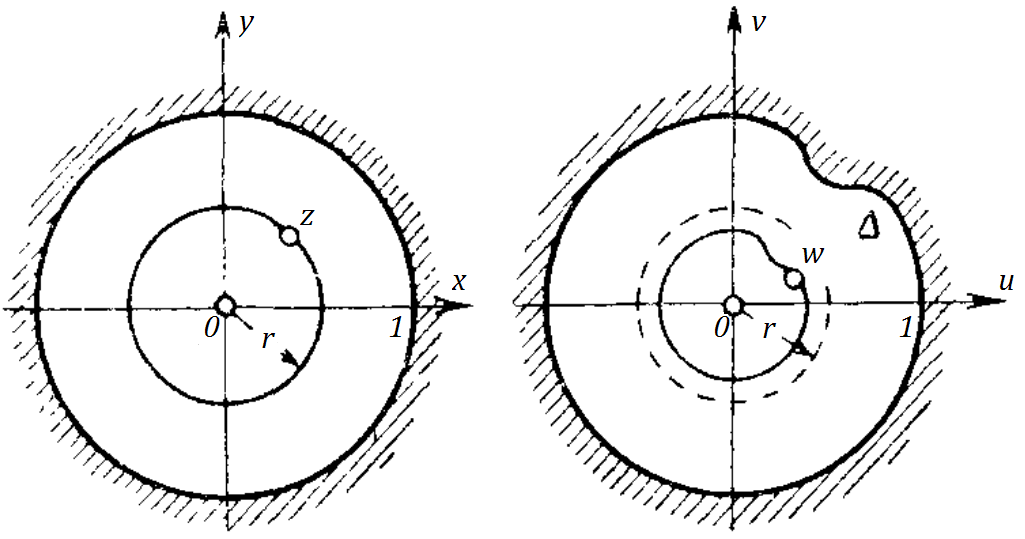
\includegraphics[width=.8\linewidth]{mal-25.png}
	%\caption{Геометричний зміст леми Шварца.}
\end{figure}


% \setcounter{subsection}{15}
\subsection{Рівномірна збіжність}
Цей пункт має допоміжний характер. У ньому ми розглянемо важливі питання, пов'язані з рівномірною збіжністю послідовностей і рядів аналітичних функцій. \\

Послідовність функцій $f_1(z)$, $f_2(z)$, $\ldots$ називається \textit{рівномірно збіжною} до функції $f(z)$ в області $D$ (або на кривій $C$), якщо для довільного $\epsilon > 0$ знайдеться число $n_0$, яке залежить тільки від $\epsilon$ таке, що для всіх $n > n_0$ і всіх $z$ із $D$ (або на $C$) виконується нерівність
\begin{equation}
	\label{eq:4.6.1}
	|f_n(z) - f(z)| < \epsilon.
\end{equation}

Доведемо дві теореми, аналогічні відповідним теоремам аналізу.

\begin{theorem}
\label{th:4.6.1}
Границя $f(z)$ послідовності неперервних функцій $f_1(z)$, $f_2(z)$, $\ldots$, яка рівномірно сходиться в деякій області $D$ (або на кривій $C$) також є неперервною функцією.
\end{theorem}

\begin{proof}
Зафіксуємо $\epsilon > 0$ і довільну точку $z_0$ області $D$ (або кривої $C$). Завдяки рівномірній збіжності знайдеться $n$ таке, що для всіх $z$ із $D$ (на $C$):
\begin{equation}
	\label{eq:4.6.2}
	|f(z) - f_n(z)| < \dfrac{\epsilon}{3}.
\end{equation}
Завдяки неперервності $f_n(z)$ в точці $z_0$ знайдеться те число $\delta > 0$, що для всіх $z$ із $D$ (на $C$), що задовольняють нерівність $|z - z_0| < \delta$ виконується нерівність
\begin{equation}
	\label{eq:4.6.3}
	|f_n(z) - f_n(z_0)| < \dfrac{\epsilon}{3}.
\end{equation}
Для таких $z$ і вибраного вище $n$ з нерівностей \eqref{eq:4.6.2} і \eqref{eq:4.6.3} маємо:
\begin{multline}
	\label{eq:4.6.4}
	|f(z) - f(z_0)| \le |f(z) - f_n(z)| + |f_n(z) - f_n(z_0)| + \\ + |f_n(z_0) - f(z_0)| \le \dfrac{\epsilon}{3} + \dfrac{\epsilon}{3} + \dfrac{\epsilon}{3} = \epsilon,
\end{multline} а це й означає неперервність $f(z)$.
\end{proof}

\begin{theorem}
	\label{th:4.6.2}
	Якщо послідовність неперервних функцій $f_1(z)$, $f_2(z)$, $\ldots$ на кривій $C$ рівномірно сходиться до $f(z)$, то виконується граничне співвідношення
	\begin{equation}
		\label{eq:4.6.5}
		\Lim_{n \to \infty} \Int_C f_n(z) \diff z = \Int_C \Lim_{n \to \infty} f_n(z) \diff z.
	\end{equation}
\end{theorem}

\begin{proof}
Зафіксуємо $\epsilon > 0$. Завдяки рівномірній збіжності знайдеться таке $n_0$ що для всіх $n > n_0$ і для всіх $z$ на $C$:
\begin{equation}
	\label{eq:4.6.6}
	|f_n(z) - f(z)| \le \dfrac{\epsilon}{l},
\end{equation}
де $l$ -- довжина $C$. Для таких $n$:
\begin{equation}
	\label{eq:4.6.7}
	\left| \Int_C f(z) \diff z - \Int_C f_n(z) \diff z \right| = \left| \Int_C (f(z) - f_n(z)) \diff z \right| < \dfrac{\epsilon}{l} l = \epsilon,
\end{equation}
а це і означає справедливість співвідношення \eqref{eq:4.6.5}.
\end{proof}

Доведена теорема надає можливість переходити до границі під знаком інтегралу у випадку рівномірної збіжності послідовності функцій. \\

З поняттям рівномірної збіжності послідовності тісно пов'язане поняття рівномірно збіжного ряду. Функціональний ряд $\sum_{n = 0}^\infty f_n(z)$ називається \textit{рівномірно збіжним} в області $D$ (на кривій $C$) якщо послідовність його частинних сум рівномірно збіжна в цій області (на цій кривій). \\

Так само як і в аналізі, доводиться зручна для застосування достатня ознака рівномірної збіжності функціональних рядів.

\begin{theorem}
	\label{th:4.6.3}
	Якщо функціональний ряд $\sum_{n = 0}^\infty f_n(z)$ в області $D$ мажорується збіжним числовим рядом $\sum_{n = 0}^\infty a_n$, тобто для довільної точки $z$ із $D$
	\begin{equation}
		\label{eq:4.6.8}
		|f_n(z)| \le a_n \quad (n = 0, 1, 2, \ldots),
	\end{equation}
	то цей функціональний ряд рівномірно збіжний в $D$.
\end{theorem}

\begin{proof}
Справді, за відомою теоремою порівняння цей ряд збіжний в довільній точці $z$ із $D$. Позначимо його суму через $s(z)$. Для довільного $n$ залишок $r_n(z) = s(z) - s_n(z)$ цього ряду завдяки співвідношенню \eqref{eq:4.6.8} задовольняє нерівності
\begin{equation}
	\label{eq:4.6.9}
	|r_n(z)| \le |f_{n + 1}(z)| + |f_{n + 2}(z)| + \ldots \le a_{n + 1} + a_{n + 2} + \ldots
\end{equation}
Права сторона цієї нерівності є залишком $r_n$ збіжного числового ряду, тобто прямує до $0$ при $n \to \infty$. Як наслідок, для довільного $\epsilon > 0$ можна знайти $n_0$ яке залежить лише від $\epsilon$ починаючи з якого $r_n < \epsilon$. Тоді, завдяки \eqref{eq:4.6.9} для довільного $z$ із $D$ і $n > n_0$ буде виконуватися нерівність
\begin{equation}
	\label{eq:4.6.10}
	|s(z) - s_n(z)| < \epsilon,
\end{equation} а це й означає рівномірну збіжність ряду.
\end{proof}

З теорем \ref{th:4.16.1} і \ref{th:4.16.2} випливає, що сума рівномірно збіжного ряду, що складається з неперервних функцій неперервна, і що такий ряд можна почленно інтегрувати, тобто що справджується співвідношення
\begin{equation}
	\label{eq:4.6.11}
	\Sum_{n = 0}^\infty \Int_C f_n(z) \diff z = \Int_C \Sum_{n = 0}^\infty f_n(z) \diff z.
\end{equation}

Питання про можливість почленного диференціювання функціональних рядів буде розглянуто у пункті 5.2 (теорема Веєрштрасса). \\

Розглянемо тепер сім'ю функцій $f(z, \alpha)$ що залежать від параметра (дійсного чи комплексного) $\alpha$. Кажуть, що $f(z, \alpha)$ прямує при $\alpha \to \alpha_0$ до функції $f(z)$ \textit{рівномірно відносно} $z$ в області $D$ (або на кривій $C$), якщо для довільного $\epsilon > 0$ знайдеться $\delta = \delta(\epsilon)$ таке, що при $|\alpha - \alpha_0| < \delta$ для всіх $z$ з $D$ (або на $C$) виконується нерівність
\begin{equation}
	\label{eq:4.6.12}
	|f(z, \alpha) - f(z)| < \epsilon.
\end{equation}

Точно так само як і для послідовностей, можна показати, що границя рівномірно збіжної сім'ї неперервних функцій є неперервною функцією, і що для такої сім'ї справджується граничне співвідношення
\begin{equation}
	\label{eq:4.6.13}
	\Lim_{\alpha \to \alpha_0} \Int_C f(z, \alpha) \diff z = \Int_C \Lim_{\alpha \to \alpha_0} f(z, \alpha) \diff z.
\end{equation}

Надалі нам доведеться мати справу з інтегралами вздовж необмежених кривих -- \textit{невласними інтегралами}. При цьому ми завжди будемо розглядати лише такі криві $C$, відрізки який, що належать довільному кругу, є кусково-гладкими. Функції $f(z)$ задані на $C$ будемо вважати кусково-неперервними і обмеженими. \\

Визначимо тепер інтеграл від функції $f(z)$ вздовж необмеженої кривої $C$. Нехай спершу $C$ не обмежена лише в одну сторону і $a$ -- її кінець. Тоді ми позначимо через $C_l$ частину $C$ з кінцем $a$ і довжиною $l$ і покладемо за визначенням
\begin{equation}
	\label{eq:4.6.14}
	\Int_C f(z) \diff z = \Lim_{l \to \infty} \Int_{C_l} f(z) \diff z,
\end{equation}
причому, якщо ця границя існує, то будемо казати, що (невласний) інтеграл \eqref{eq:4.6.14} \textit{збіжний}. Якщо ж $C$ не обмежена в обидва боки, то визначимо інтеграл як суму інтегралів вздовж двох частин на які $C$ ділиться довільною точкою $a$. \\

Нехай функція $f(z, \zeta)$ визначена для всіх $z$ з області $D$ і для всіх $\zeta$ на лінії $C$. Будемо казати, що інтеграл
\begin{equation}
	\label{eq:4.6.15}
	F(z) = \Int_C f(z, \zeta) \diff \zeta
\end{equation}
\textit{рівномірно збіжний} в області $D$, якщо для довільного $\epsilon > 0$ знайдеться $l_0$ таке, що для всіх $z$ із $D$ при довільному $l > l_0$:
\begin{equation}
	\label{eq:4.6.16}
	\left| \Int_C f(z, \zeta) \diff \zeta - \Int_{C_l} f(z, \zeta) \diff \zeta \right| < \epsilon
\end{equation}
\begin{remark*}
Визначення у припущенні необмеженості $C$ в одну сторону, розповсюджується на необмежені в обидві сторони криві аналогічно попередньому.
\end{remark*}

\begin{theorem}
\label{th:4.6.4}
Якщо функція $f(z, \zeta)$ аналітична по $z$ і кусково неперервна по $\zeta$ для всіх $z$ з однозв'язної області $D$ і для всіх $\zeta$ на лінії $C$, і інтеграл
\begin{equation}
	\label{eq:4.6.17}
	F(z) = \Int_C f(z, \zeta) \diff \zeta
\end{equation}
збігається рівномірно в області $D$, то він є аналітичною в цій області функцією.
\end{theorem}

\begin{proof}
Для доведення скористаємося теоремою, оберненою до теореми Коші, згідно з якою функція $F(z)$ аналітична в однозв'язній області $D$ якщо вона неперервна в цій області, а її інтеграл вздовж довільної замкнутої кривої, що належить області, дорівнює нулю (доведення цієї теореми див. у наступному пункті). \\

В умовах теореми яку ми зараз доводимо неперервність функції $F(z)$ встановлюється звичним чином (як теорема \ref{th:4.6.2} або співвідношення \eqref{eq:4.6.13}). Залишається показати, що інтеграл від $F(z)$ вздовж довільного замкнутого контуру $\Gamma$, що належить області $D$, дорівнює нулю. Маємо:
\begin{equation}
	\label{eq:4.6.18}
	\Int_\Gamma F(z) \diff z = \Int_\Gamma \left( \Int_C f(z, \zeta) \diff \zeta \right) \diff z.
\end{equation}
Завдяки рівномірній збіжності інтегралу \eqref{eq:4.6.17} за відомою з аналізу теоремою, у правій частині можна змінити порядок інтегрування, і ми отримаємо:
\begin{equation}
	\label{eq:4.6.19}
	\Int_\Gamma F(z) \diff z = \Int_C \left( \Int_\Gamma f(z, \zeta) \diff z \right) \diff \zeta = 0,
\end{equation}
адже внутрішній інтеграл дорівнює нулю за теоремою Коші.
\end{proof}

Зауважимо, що у випадку обмеженої кривої $C$ для аналітичності функції $F(z)$ не потрібно жодних додаткових припущень щодо збіжності інтегралу \eqref{eq:4.6.17}, адже це випливає з можливості зміни порядку інтегрування у співвідношенні \eqref{eq:4.6.18} без додаткових припущень.


% \setcounter{subsection}{16}
\subsection{Вищі похідні}
За визначенням, аналітична функція -- це функція комплексної змінної, яка має похідну в кожній точці деякої області $D$. Покажемо, що з аналітичності функції автоматично випливає існування і аналітичність всіх її послідовних похідних.

\begin{theorem}[О. Коші, 1842 р.]
	\label{th:4.7.1}
	Якщо функція $f(z)$ аналітична в області $D$ і неперервна в $\overline{D}$, то вона має в кожній точці $D$ похідні всіх порядків, причому $n$-а похідна може бути представлена формулою
	\begin{equation}
		\label{eq:4.7.1}
		f^{(n)}(z) = \dfrac{n!}{2 \pi i} \Int_C \dfrac{f(\zeta) \diff \zeta}{(\zeta - z)^{n + 1}},
	\end{equation}
	де $C$ -- межа області $D$.
\end{theorem}


\begin{proof}
Нехай $z$ -- довільна внутрішня точка області $D$. За визначенням похідної та формулою Коші з пункту 14, яку ми застосовуємо до точок $z$ і $z + h$ маємо:
\begin{multline}
	\label{eq:4.7.2}
	f'(z) = \Lim_{h \to 0} \dfrac{f(z + h) - f(z)}{h} = \\ = \dfrac{1}{2 \pi i} \Lim_{h \to 0} \dfrac{1}{h} \Int_C f(\zeta) \left( \dfrac{1}{\zeta - z - h} - \dfrac{1}{\zeta - z} \right) = \\ = \dfrac{1}{2 \pi i} \Lim_{h \to 0} \Int_C \dfrac{f(\zeta) \diff \zeta}{(\zeta - z - h) (\zeta - z)}.
\end{multline}
Але, очевидно, що при $h \to 0$ функція $\frac{1}{\zeta - z - h}$ рівномірно для віх $\zeta$ на $C$ прямує до $\frac{1}{\zeta - z}$, і, як наслідок, за теоремою \ref{th:4.6.2}, границя існує, причому
\begin{equation}
	\label{eq:4.7.3}
	f'(z) = \dfrac{1}{2 \pi i} \Int_C \dfrac{f(\zeta) \diff \zeta}{(\zeta - z)^2}.
\end{equation}
Для $n = 1$ теорема доведена. Далі теорема доводиться методом математичної індукції.
\end{proof}

\begin{remark*}
	Як видно з доведення, теорему можна сформулювати ще наступним чином: якщо функція $\phi(\zeta)$ неперервна на межі $C$ області $D$, то функція
	\begin{equation}
		\label{eq:4.7.4}
		f(z) = \dfrac{1}{2 \pi i} \Int_C \dfrac{\phi(\zeta) \diff \zeta}{\zeta - z},
	\end{equation}
	що задається формулою Коші, аналітична в цій області.
\end{remark*}

\begin{remark*}
	Формули \eqref{eq:4.7.1} для похідних можна отримати формальним диференціюванням формули Коші по $z$. Доведена теорема стверджує законність цього диференціювання.
\end{remark*}

З формули \eqref{eq:4.7.1} випливають важливі \textit{нерівності Коші}. Позначимо через $M$ максимум модуля функції $f(z)$ в області $D$, через $R$ -- відстань від точки $z$ до межі області $D$ і через $l$ -- довжину цієї межі. З \eqref{eq:4.7.1} маємо:
\begin{equation}
	\label{eq:4.7.5}
	|f^{(n)}(z)| \le \dfrac{n!}{2 \pi} \left| \Int_C \dfrac{f(\zeta) \diff \zeta}{(\zeta - z)^{n + 1}} \right| \le \dfrac{n! M l}{2 \pi R^{n + 1}}.
\end{equation}
Якщо, зокрема, $f(z)$ аналітична в крузі $|z - z_0| < R$, то, взявши в ролі $D$ цей круг, отримаємо
\begin{equation}
	\label{eq:4.7.6}
	|f^{(n)}(z_0)| \le \dfrac{M n!}{R^n}, \quad n = 0, 1, 2, \ldots
\end{equation}
Це і є нерівності Коші, які ми хотіли довести. \\

Скористаємося отриманими результатами для доведення двох важливих теорем теорії аналітичних функцій.

\begin{theorem}[Ж. Ліувіль]
	\label{th:4.7.2}
	Якщо функція $f(z)$ аналітична у всій площині та обмежена то вона стала.
\end{theorem}
\begin{proof}
Нехай всюди $|f(z)| \le M$. Для довільної точки $z$ площини та для довільного $R$ нерівність \eqref{eq:4.7.6} при $n = 1$ дає:
\begin{equation}
	\label{eq:4.7.7}
	|f'(z)| \le \dfrac{M}{R} \xrightarrow[R \to \infty]{} 0.
\end{equation}
Але ліва частина не залежить від $R$, ому вона просто дорівнює нулю, тобто $|f'(z)| = 0$, або $f'(z) \equiv 0$ у всій площині. Звідси, за теоремою \ref{th:4.2.4} робимо висновок, що
\begin{equation}
	\label{eq:4.7.8}
	f(z) - f(z_0) = \Int_{z_0}^z f'(z) \diff z \equiv 0,
\end{equation}
тобто що функція $f(z)$ стала.
\end{proof}

\begin{remark*}
	Теорема \ref{th:4.7.2} може бути узагальнена наступним чином: \\

	Нехай функція $f(z)$ аналітична у всі площині, і її модуль зростає не швидше ніж $M\cdot|z|^n$, де $n$ -- ціле число, а $M$ -- стала, то ця функція є поліномом степені не вище $n$. \\

	Доведення аналогічне попередньому: нехай $z_0$ -- довільна точка площини; з нерівності \eqref{eq:4.7.6} маємо
	\begin{equation}
		\label{eq:4.7.9}
		\left| f^{(n + 1)}(z_0) \right| \le \frac{M \cdot |z|^n}{R^{n + 1}} \cdot (n + 1)!
	\end{equation}
	і, помічаючи, що у нас $|z| \le |z_0| + R$, після переходу до границі при $R \to \infty$ отримуємо, що $f^{(n + 1)}(z_0) = 0$. Оскільки $z_0$ -- довільна точка площини, то $f^{(n + 1)}(z) \equiv 0$, а звідси тим же методом, що і вище, нескладно прийти до бажаного результату.
\end{remark*}
Наступна теорема обернена до основної теореми Коші з пункту 12.

\begin{theorem}[Г. Морера, 1886 р.]
	\label{th:4.7.3}
	Якщо функція $f(z)$ неперервна в однозв'язній області $D$ і інтеграл $\int_C f(z) \diff z$ по довільному замкнутому контуру, що лежить в $D$, дорівнює 0, то $f(z)$ аналітична в цій області.
\end{theorem}

\begin{proof}
З умов теореми випливає, що в області $D$ інтеграл $\int_{z_0}^z f(z) \diff z$ не залежить від шляху інтегрування, тобто для фіксованого $z_0$ він визначає деяку функцію $z$:
\begin{equation}
	\label{eq:4.7.10}
	F(z) = \Int_{z_0}^z f(z) \diff z.
\end{equation}
Повторюючи доведення теореми \ref{th:4.2.2}, ми побачимо, що ця функція має похідну $F'(z) = f(z)$, тобто аналітична. Але тоді за теоремою \ref{th:4.7.1}, $f(z)$ є аналітичною функцією як похідна аналітичної функції.
\end{proof}

% \flushright{\copyright \, М. А. Лаврентьев, Б. В. Шабат, 1972 \\ Українською переклав Н. М. Скибицький, 2018}

% \end{document}